%******************** MODE EXPANSION *********************
\section{Mode Expansion}\label{sec:bosonic-mode-expansion}
We use mostly plus metric $\eta = \textup{diag}(-,+,\dots,+)$ and focus on \emph{closed strings}. We already focus on the \emph{critical string}, considering as a background the flat $26d$ Minkowski spacetime $\M_{26}$.

The worldsheet coordinates are $\xi^a = (\tau, \sigma)$, $a= 1,2$, where $\sigma \in (0,l)$. Taking as a background the flat $26$-dimensional Minkowski spacetime $\M_{26}$, the string is described by the worldsheet fields $X^{{\mu}}$, with ${\mu} = 0, \dots, 25$. Considering the $2d$ metric $\gamma_{ab}(\xi^a)$, the Polyakov action reads
\begin{equation}\label{eq:polyakov-action}
    S_P= -\frac{1}{4\pi\alpha'} \int_\Sigma \ud^2 \xi \sqrt{-\gamma} \, \gamma^{ab} \de_a X^{{\mu}} \de_b X^{{\nu}} \eta_{{\mu}{\nu}} ,
\end{equation}
where the string tension is
\begin{equation}
    T = \frac{1}{2\pi\alpha'} .
\end{equation}

Exploiting the reparametrisation invariance and the Weyl symmetry, we can go to \emph{conformal gauge}, in which $\gamma_{ab} = \eta_{ab}$, such that Polyakov action becomes
\begin{equation}\label{eq:polyakov-conformal-gauge}
    S_P= -\frac{1}{4\pi\alpha'} \int_\Sigma \ud^2 \xi \, \de_a X^{{\mu}} \de^a X_{{\nu}}  .
\end{equation}

Defining \emph{worldsheet lightcone coordinates} $\xi^\pm \equiv \tau \pm \sigma$, the equations of motion read $\de_+\de_- X^\mu = 0$, which is solved by the ansatz
\begin{equation}\label{eq:left-right-movers-def}
    X^{{\mu}}(\xi^a) = X^{{\mu}}_L(\xi^+) + X^{{\mu}}_R(\xi^-) ,
\end{equation}
where $\xi^\pm \equiv \tau \pm \sigma$. For a closed string, we must further impose the boundary condition
\begin{equation}\label{eq:boundary-condition}
    X^\mu (\tau,\sigma) = X^\mu (\tau, \sigma + l),
\end{equation}
which is compatible with~\eqref{eq:left-right-movers-def} for the following mode decomposition
\begin{subequations}\label{eq:mode-expansion}
\begin{align}
    X^\mu_L(\xi^+) &= \frac{x^\mu}{2} + \sqrt{2\alpha'} \frac{\pi}{l} \tilde{\alpha}^\mu_0 \xi^+ + i \sqrt{\frac{\alpha'}{2}} \sum_{n\neq 0} \frac{\tilde{\alpha}^\mu_n}{n}e^{-\frac{2\pi i}{l}n \xi^+} \\
    X^\mu_R(\xi^-) &= \frac{x^\mu}{2} + \sqrt{2\alpha'} \frac{\pi}{l} {\alpha}^\mu_0 \xi^- + i \sqrt{\frac{\alpha'}{2}} \sum_{n\neq 0} \frac{{\alpha}^\mu_n}{n}e^{-\frac{2\pi i}{l}n \xi^-} .
\end{align}
\end{subequations}

Summing them, we find
\begin{equation}\label{eq:generic-expansion}
    X^\mu (\tau,\sigma) = x^\mu + \sqrt{2\alpha'} \frac{\pi}{l} (\tilde{\alpha}^\mu_0 + \alpha^\mu_0) \tau + \sqrt{2\alpha'} \frac{\pi}{l} (\tilde{\alpha}^\mu_0 - \alpha^\mu_0) \sigma + \textup{oscillators},
\end{equation}
which, under $\sigma \to \sigma + l$, transforms as $\delta X^\mu = \sqrt{2\alpha'}\frac{\pi}{l}(\tilde{\alpha}^\mu_0 - \alpha^\mu_0) l \overset{\mathrm{!}}{=} 0$. So, to satisfy the boundary condition~\eqref{eq:boundary-condition}, it must be $\alpha^\mu_0 = \tilde{\alpha}^\mu_0$. Moreover, using Noether's theorem for the global Poincaré symmetry, the charge conserved under translations $\delta X^\mu = \epsilon^\mu$ is 
\begin{equation}\label{eq:noteher-momentum}
    \frac{1}{\sqrt{2\alpha'}} (\tilde{\alpha}^\mu_0 + \alpha^\mu_0) \equiv p^\mu,
\end{equation}
so
\begin{equation}\label{eq:relation-alpha-momentum}
    \alpha^\mu_0 = \tilde{\alpha}^\mu_0 = \sqrt{\frac{\alpha'}{2}}p^\mu .
\end{equation}

\begin{mdframed}
\begin{innerproof}
    Under a transformation
    \begin{equation}
        \phi_k(x) \to \phi_k(x) + \epsilon \Delta\phi_k(x) + O(\epsilon^2),
    \end{equation}
    the lagrangian transforms as $\L \to \L + \Delta \L$, with
    \begin{equation}
        \Delta \L = \frac{\de \L}{\de \phi_k} (\epsilon \Delta \phi_k) + \frac{\de \L}{\de(\de_\mu \phi_k)} \de_\mu (\epsilon \Delta \phi_k) .
    \end{equation}
    After integration by parts and using the equations of motion, we easily see that the conserved current, such that $\de_\mu J^\mu = 0$ is
    \begin{equation}
        J^\mu = \frac{\de \L}{\de(\de_\mu \phi_k)} \Delta \phi_k - k^\mu
    \end{equation}
    Considering Polyakov action in conformal gauge, 
    \begin{equation}
    S_P = -\frac{1}{4\pi\alpha'}\int \ud^2 \, \xi \de_a X\cdot \de^a X,
    \end{equation}
    we can compute
    \begin{equation*}
        \delta X^\mu = \epsilon^\mu, \quad \frac{\de \L}{\de(\de^a X_\mu)} = - \frac{1}{2\pi\alpha'} \de_a X^\mu, \quad q_a = -\frac{1}{2\pi\alpha'} \de_a X^\mu \epsilon_\mu.
    \end{equation*}
    So, the conserved current is
    \begin{equation}
        q^\mu_a = - \frac{1}{2\pi\alpha'} \de_a X^\mu,
    \end{equation}
    and the conserved charge is, up to a sign
    \begin{equation}
        p^\mu \equiv  -\int_0^l \ud \sigma (q^\mu)_\tau = \frac{1}{2\pi\alpha'} \de_\tau X^\mu.
    \end{equation}
    Using, then, the mode decomposition~\eqref{eq:mode-expansion}, giving that the spacial integral of the oscillators' exponentials vanish, we get
    \begin{equation}
        p^\mu = \frac{1}{2\pi\alpha'} \int_0^l \ud \sigma \, \sqrt{2\alpha'} \frac{\pi}{l} (\tilde{\alpha}^\mu_0 + \alpha^\mu_0) + \dots = \frac{1}{\sqrt{2\alpha'}} (\tilde{\alpha}^\mu_0 + \alpha^\mu_0).
    \end{equation}
\end{innerproof}
\end{mdframed}


%******************** LIGHTCONE GAUGE *********************
\section{Lightcone Gauge}
In lightcone quantization, we impose the Virasoro constraints $T_{ab}=0$ on the classical theory. In worldsheet lightcone coordinates, they ensure that the reparametrizations
\begin{equation}\label{eq:reparam}
    \xi^+ \to \tilde{\xi}^+(\xi^+), \quad \xi^- \to \tilde{\xi}^-(\xi^-),
\end{equation}
which induce a conformal transformation, is a gauge symmetry of the classical theory. It's convenient to define \emph{spacetie lightcone coordinates}
\begin{equation}
    X^\pm = \frac{1}{\sqrt{2}}(X^0 \pm X^1), \quad X^i, i = 2, \dots, 25,
\end{equation}
so that, the above freedom~\eqref{eq:reparam} can be used to fix
\begin{equation}\label{eq:choice-x+}
    X^+(\tau,\sigma) = x^+ + \frac{2\pi\alpha'}{l}p^+ \tau ,
\end{equation}
wihch is called \emph{lightcone gauge}. Then, the mode expansion~\eqref{eq:mode-expansion}, with~\eqref{eq:relation-alpha-momentum}, would be, in lightcone gauge,
\begin{subequations}
\begin{align}
    X^+_L(\xi^+) &= \frac{x^+}{2} + \frac{\pi\alpha'}{l}p^+ \xi^+, \\
    X^+_R(\xi^-) &= \frac{x^+}{2} + \frac{\pi\alpha'}{l}p^+ \xi^-, \\
    X^-_L(\xi^+) &= \frac{1}{2} x^- + \frac{\pi\alpha'}{l} p^- \xi^+ + i \sqrt{\frac{\alpha'}{2}} \sum_{n\neq 0}\frac{\tilde{\alpha}^-_n}{n} e^{-\frac{2\pi i}{l}n \xi^+}, \\
    X^-_R(\xi^-) &=\frac{1}{2} x^- + \frac{\pi\alpha'}{l} p^- \xi^- + i \sqrt{\frac{\alpha'}{2}} \sum_{n\neq 0}\frac{{\alpha}^-_n}{n} e^{-\frac{2\pi i}{l}n \xi^-},
\end{align}
\end{subequations}
where, in particular, the constraints $T_{ab}=0$ with the choice~\eqref{eq:choice-x+}, fix all the $\alpha^-$ and $\tilde{\alpha}^-$ modes in terms of the $\alpha^i$ and $\tilde{\alpha}^i$, via the relations\footnote{Details in Ling Lin's notes. We're not interested in those here.}
\begin{equation}\label{eq:relation-alpha--}
    \tilde{\alpha}^-_n = \frac{1}{\sqrt{2\alpha'}p^+} \sum_{m \in \Z} \tilde{\alpha}^i_{n-m} \tilde{\alpha}^i_m, \quad {\alpha}^-_n = \frac{1}{\sqrt{2\alpha'}p^+} \sum_{m \in \Z} {\alpha}^i_{n-m} {\alpha}^i_m .
\end{equation}
In this whole document, unless otherwise stated, repeated $i$-indices are summed over, with $i=2, \dots 25$.

Since the oscillators are fixed, the only remaining degree of freedom for $X^-$ is the centre of mass position,
\begin{equation}\label{eq:position-centre-mass}
   q^-(\tau) \equiv \frac{1}{l} \int_0^l \ud \sigma X^-(\tau, \sigma) ,
\end{equation}
as we'll also see writing down the action and the hamiltonian.

The Polyakov action~\eqref{eq:polyakov-conformal-gauge} reads
\begin{equation}\label{eq:lightcone-polyakov}
    S = \frac{1}{4\pi\alpha'} \int \ud \tau \ud \sigma \left( (\de_\tau X^i)^2 - (\de_\sigma X^i)^2 \right) - \int \ud \tau p^+ \de_\tau q^-,
\end{equation}
where $q^-$ is defined by~\eqref{eq:position-centre-mass}

\begin{mdframed}
\begin{innerproof}
    \begin{equation*}
    \begin{split}
        S &= -\frac{1}{4\pi\alpha'} \int \ud \tau \int_0^l \ud \sigma (\de_a X) \cdot (\de^a X) \\
        &= - \frac{1}{4\pi\alpha'} \int \ud \tau \int_0^l \ud \sigma \left( -2 \de_a X^+ \de^a X^- + \de_a X^i \de^a X^i \right) \\
        &= \frac{1}{4\pi\alpha'} \int \ud \tau \int_0^l \ud \sigma \left( (\de_\tau X^i)^2 - (\de_\sigma X^i)^2 \right) - \frac{1}{2\pi\alpha'} \int \ud \tau \int_0^l \ud \sigma \de_\tau X^+ \de_\tau X^- .
    \end{split}
    \end{equation*}
    Now, using that $\de_\tau X^+ = \frac{2\pi\alpha'}{l} p^+$, bringing it outside the spacial integral and further exchanging $\int_0^l \ud \sigma$ with $\de_\tau$ for $X^-$, we can rewrite the second part of the last expression as
    \begin{equation*}
        -\frac{1}{l} \int \ud \tau \de_\tau p^+ \left( \int_0^l \ud \sigma X^- \right) = - \int \ud \tau p^+ \de_\tau q^-,
    \end{equation*}
    where we used the definition~\eqref{eq:position-centre-mass}. Putting all together, we obtain~\eqref{eq:lightcone-polyakov}
\end{innerproof}
\end{mdframed}

From the lagrangian~\eqref{eq:lightcone-polyakov}, it's easy to compute the conjugate momenta\footnote{Pay attention that the first piece of~\eqref{eq:lightcone-polyakov} contains the lagrangian density, integrated over $\ud^2 \xi$, while the second piece is a standard lagrangian, integrated over $\ud t$. So, to find the Hamiltonian, we have to integrate over $\ud \sigma$ the conjugate momentum $\Pi_i$ to $X^i$.} to $q^-$ and $X^i$
\begin{subequations}\label{eq:conjugate-momenta}
\begin{align}
    q^i: \quad p_- &\equiv \frac{\de L}{\de(\de_\tau q^-)} = - p^+, \\
    X^i: \quad \Pi_i &\equiv \frac{\de \L}{\de(\de_\tau X^i)} = \frac{1}{2\pi\alpha'} \de_\tau X^i .
\end{align}
\end{subequations}
The Hamiltonian reads
\begin{equation}\label{eq:lightcone-hamiltonian}
\begin{split}
    H &= p_- \de_\tau q^- + \int_0^l \ud \sigma \Pi_i \de_\tau X^i - L \\
    &= \frac{1}{4\pi\alpha'} \int_0^l \ud \sigma \left[ (\de_\tau X^i)^2 + (\de_\sigma X^i)^2 \right] \\ 
    &= \frac{1}{2} \int_0^l \ud \sigma \left[ 2\pi\alpha' \Pi_i \Pi_i + \frac{1}{2\pi\alpha'} \de_\sigma X^i \de_\sigma X^i \right],
\end{split}
\end{equation}
where we used~\eqref{eq:conjugate-momenta} and, looking at~\eqref{eq:lightcone-polyakov}, the lagrangian\footnote{Here we mean the standard lagrangian, and \emph{not} the lagrangian density.}
\begin{equation}
    L = \frac{1}{4\pi\alpha'} \int_0^l \ud \sigma \left[ (\de_\tau X^i)^2 - (\de_\sigma X^i)^2 \right] - p^+ \de_\tau q^- .
\end{equation}


%******************** LIGHTCONE QUANTIZATION *********************
\section{Lightcone Quantization}\label{sec:bosonic-quant}
Observing that the conjugate variables $(X^i, \Pi_i)$ and $(q^-,p_- = - p^+)$ satisfy canonical Poisson bracket relations, we can promote them to operators acting on a Hilbert space, with commutation relations
\begin{gather}
    \comm{\alpha^i_m}{\alpha^j_n} = \comm{\tilde{\alpha}^i_m}{\tilde{\alpha}^j_n} = m \delta_{n+m,0} \delta^{ij} \\
    \comm{x^i}{p^i} = i \delta^{ij}, \quad \comm{p^+}{q^-} = i .
\end{gather}

In lightcone gauge, we completely removed the oscillators $\alpha^+_n$ and $\tilde{\alpha}^+_n$, while the $\alpha^-_n$ ($\tilde{\alpha}^-_n$) are functions of $\alpha^i_n$ ($\tilde{\alpha}^i_n$) via eq.~\eqref{eq:relation-alpha--}. Therefore, there's a normal ordering ambiguity for $n=0$, since $\comm{\alpha^i_{n-m}}{\alpha^i_m} = 0$ for $n \neq 0$. We can relate $\alpha^-_n$ to the normal ordered expression by
\begin{equation}\label{eq:minus-oscillators}
\begin{aligned}
    \alpha^-_n &= \frac{1}{\sqrt{2\alpha'}} \frac{1}{p^+} \left( \normord{\sum_{m \in \Z} \alpha^i_{n-m} \alpha^i_m} - 2 a \delta_{n,0} \right) \\
    \tilde{\alpha}^-_n &= \frac{1}{\sqrt{2\alpha'}} \frac{1}{p^+} \left( \normord{\sum_{m \in \Z} \tilde{\alpha}^i_{n-m} \tilde{\alpha}^i_m} - 2 \tilde{a} \delta_{n,0} \right) 
\end{aligned}
\end{equation}
where $a$ and $\tilde{a}$ are the normal ordering constants. The factor $2$ appears to be consistent with the usual definition of $a$, that is, to be consistent with
\begin{equation}
    \frac{1}{2} \sum_{n\neq 0} \alpha^i_{-n} \alpha^i_n = \sum_{n>0} \alpha^i_{-n} \alpha^i_n - a, \quad \frac{1}{2} \sum_{n\neq 0} \tilde{\alpha}^i_{-n} \tilde{\alpha}^i_n = \sum_{n>0} \tilde{\alpha}^i_{-n} \tilde{\alpha}^i_n - a
\end{equation}
which, after regularization, gives $a = 1$ and $\tilde{a}=1$. Further, gravitational anomaly arguments leads to $a=\tilde{a}$, so that, at the end
\begin{equation}\label{eq:ordering-constants}
    a = \tilde{a} = 1.
\end{equation}

The oscillators $\alpha^i_m$ and $\tilde{\alpha}^i_m$ are creation (for $m < 0$) and annihilation (for $m>0$) operators and $( (x^i,p_i),(q^-,p_-) )$ form $25$ Heisenberg pairs. Therefore, the vacuum is $\ket{0,k}$, where $k$ has $25$ components, being eigenvalues of $(p_-,p^i)$. Then, physical states are created by applying creation operators $\alpha^i_{m<0}$ and $\tilde{\alpha}^i_{m<0}$ in all possible ways.

Moreover, after defining the \emph{transverse number operators}
\begin{equation}\label{eq:def-transverse-number-op}
    \quad \tilde{N}_\perp \equiv \sum_{i=2}^{25}\sum_{n>0} \tilde{\alpha}^i_{-n} \tilde{\alpha}^i_n, \quad {N}_\perp \equiv \sum_{i=2}^{25}\sum_{n>0} {\alpha}^i_{-n} {\alpha}^i_n ,
\end{equation}
a careful rewriting of~\eqref{eq:minus-oscillators} leads to the \emph{level matching condition}
\begin{equation}\label{eq:level-matching}
    \tilde{N}_\perp =  N_\perp
\end{equation}
and to the \emph{mass-shell condition}
\begin{equation}\label{eq:mass-shell}
    M^2 = \frac{2}{\alpha'} (\tilde{N}_\perp + N_\perp - 2) .
\end{equation}

\begin{mdframed}
\begin{innerproof}
    Let's consider~\eqref{eq:minus-oscillators} for $n=0$, and use ~\eqref{eq:relation-alpha-momentum}, i.e., $\alpha^-_0 = \tilde{\alpha}^-_0 = \sqrt{\frac{\alpha'}{2}} p^-$ and $\alpha^i_0 = \tilde{\alpha}^i_0 = \sqrt{\frac{\alpha'}{2}}p^i$. We get
    \begin{equation}
    \begin{aligned}
        \alpha' p^- p^+ &= \frac{\alpha'}{2} p^i p^i + \normord{\sum_{n\neq0} \alpha^i_{-n} \alpha^i_n} - 2 = \frac{\alpha'}{2} p^i p^i + 2 \sum_{n>0} \alpha^i_{-n} \alpha^i_n - 2, \\
        \alpha' p^- p^+ &= \frac{\alpha'}{2} p^i p^i + \normord{\sum_{n\neq0} \tilde{\alpha}^i_{-n} \tilde{\alpha}^i_n} - 2 = \frac{\alpha'}{2} p^i p^i + 2{\sum_{n>0} \tilde{\alpha}^i_{-n} \tilde{\alpha}^i_n} - 2 ,\\
    \end{aligned}
    \end{equation}
    where we used~\eqref{eq:ordering-constants} and the definition of normal ordering. Therefore, by means of~\eqref{eq:def-transverse-number-op}, we get $\tilde{N}_\perp = N_\perp$. Further, dividing by $\alpha'$ and summing the above equations yields
    \begin{equation}
        2 p^+ p^- = p^i p^i + \frac{2}{\alpha'} (N_\perp + \tilde{N}_\perp) - \frac{4}{\alpha'},
    \end{equation}
    which can be used to compute
    \begin{equation}
        M^2 = - p_\mu p^\mu = 2p^+ p^- - p^i p^i = \frac{2}{\alpha'} (\tilde{N}_\perp + N_\perp - 2),
    \end{equation}
    as claimed.
\end{innerproof}
\end{mdframed}

%**************** COMPACTIFICATION ON S^1 *****************+ 
\section{Compactification on \texorpdfstring{$S^1$}{S1}}
Let's now focus on \emph{closed strings} and compactify $\M_{26}$ on $\M_{25} \times S^1$.

We'll refer to lightcone quantization, with the only difference being the name of the indices. In particular, we'll denote with $\hat{\mu}$ the indices of $\M_{26}$, with $\hat{\mu} = 0, \dots, 25$, and with $\mu$ the indices of $\M_{25}$, with $\mu = 0, \dots , 24$. This means that we can write $X^{\hat{\mu}} = (X^\mu, X^{25})$. Similarly, the transversal indices will be called $\hat{i}$ in the following, with $\hat{i} = 2, \dots 25$, while $i$ will denote the transversal indices in the non-compact space $\M_{25}$, with $i = 2, \dots 24$. Therefore, in spacetime lightcone coordinates, we have $X^{\hat{\mu}} \to (X^\pm, X^{\hat{i}}) = (X^\pm, X^i, X^{25})$.

The dynamics of the strings oscillations is \emph{locally} identical for the theory on $\M_{26}$ and $\M_{25} \times S^1$. Indeed, the difference is in a global effect, i.e., the identification $x^{25} = y \simeq y + 2\pi R$. Therefore, the local dynamics is still described by the action~\eqref{eq:lightcone-polyakov}, i.e.,
\begin{equation}
    S = \frac{1}{4\pi\alpha'} \int \ud \tau \ud \sigma \left( (\de_\tau X^{\hat{i}})^2 - (\de_\sigma X^{\hat{i}})^2 \right) - \int \ud \tau p^+ \de_\tau q^-,
\end{equation}
with the difference being the boundary conditions of the worldsheet fields. Then, in lightcone quantization, the relevant degrees of freedom are still $X^{\hat{i}}(\tau,\sigma)$, $\hat{i} = 2, \dots, 25$, with Hamiltonian~\eqref{eq:lightcone-hamiltonian}, i.e.,
\begin{equation}
    H = \frac{1}{2} \int_0^l \ud \sigma \left[ 2\pi\alpha' \Pi_{\hat{i}} \Pi_{\hat{i}} + \frac{1}{2\pi\alpha'} \de_\sigma X^{\hat{i}} \de_\sigma X^{\hat{i}} \right],
\end{equation}

\begin{figure}
    \centering
    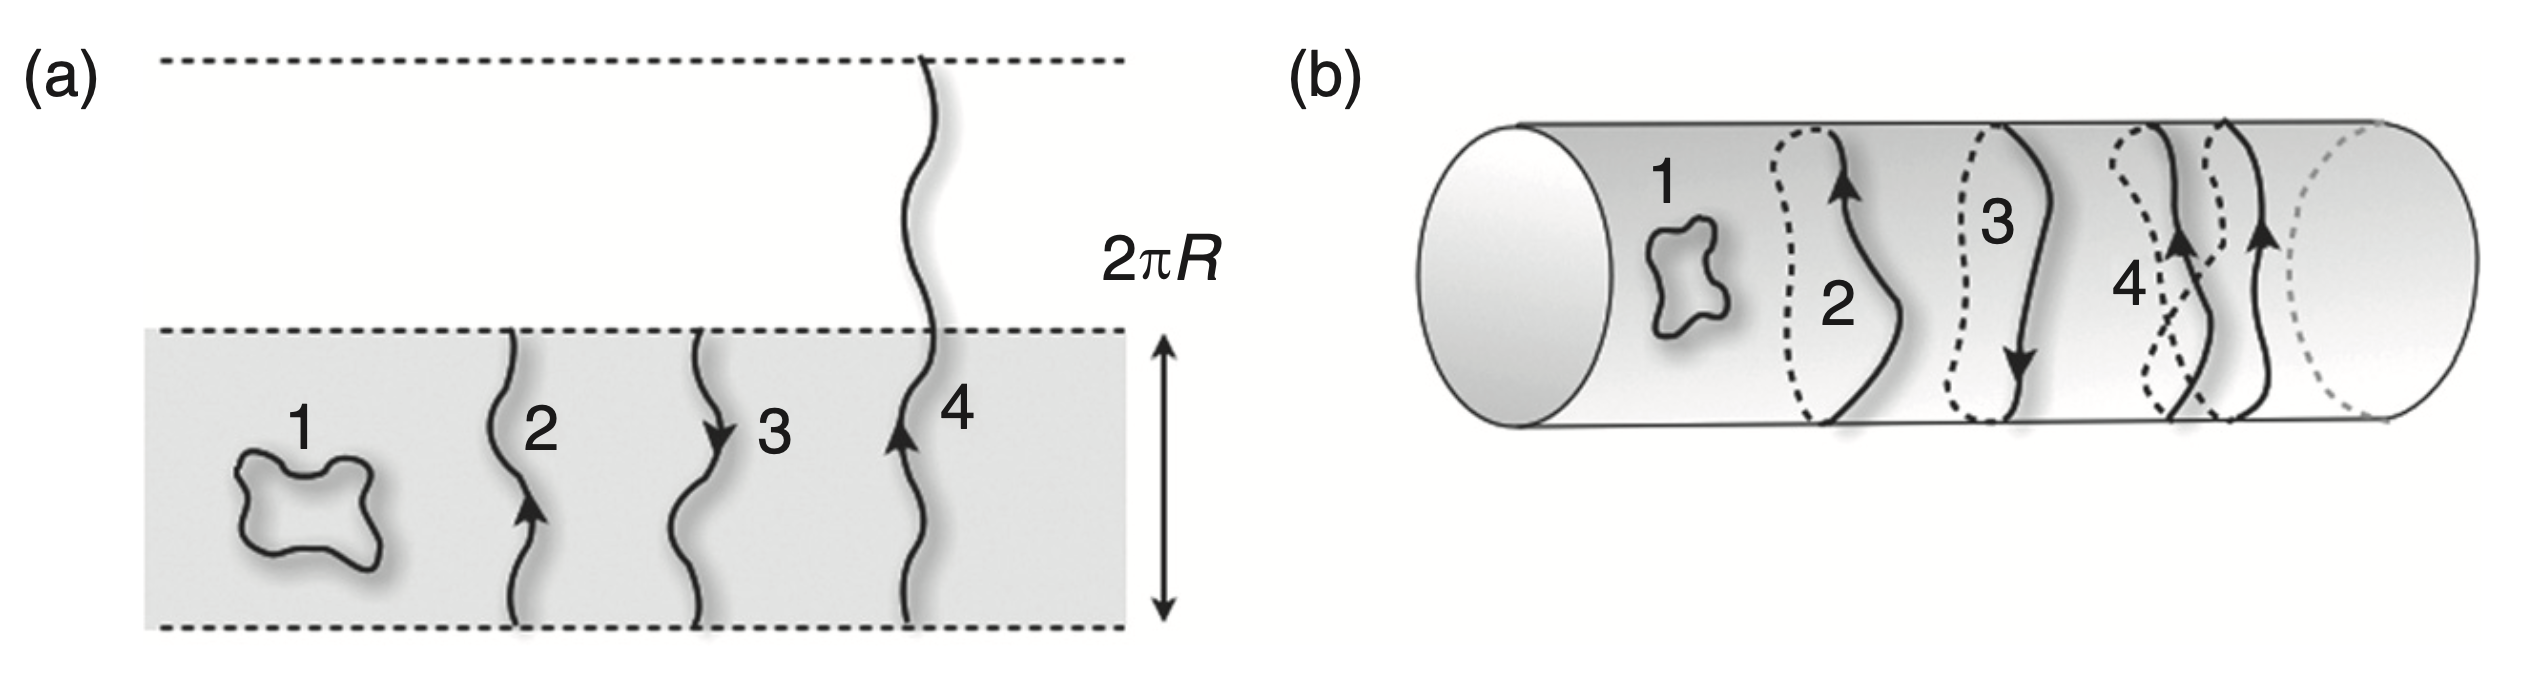
\includegraphics[width=\textwidth]{figures/winding.png}
    \caption{Closed stirng states in $S^1$ compactifications. The closed string $1$ is closed already in flat $26d$ space, and has no winding. Closed strings $2$, $3$ and $4$ are closed only after periodic identification defining the circle. States $2$ and $3$ have opposite winding numbers $\omega = \pm 1$, and state $4$ has a multiple winding $\omega = 2$.}
    \label{fig:winding}
\end{figure}

To express it in terms of the oscillator modes, we first need to specify the boundary conditions. In particular, writing $X^{\hat{i}} = (X^i, X^{25})$, we have the usual periodic boundary condition for the $X^i$ with $i = 2, \dots, 24$, while $X^{25}$ can have a more general boundary condition due to the periodicity $x^{25} = y \simeq y + 2\pi R$ in the internal space. Specifically,
\begin{subequations}
\begin{align}
    X^i(t,\sigma + l) &= X^i(t,\sigma), \quad i = 2, \dots, 24\\
    X^{25}(t,\sigma + l) &= X^{25}(t,\sigma) + 2\pi R \omega, \quad \omega \in \Z.
\end{align}
\end{subequations}
For $\omega = 0$, it describes the usual boundary condition, while for $\omega \neq 0$ it describes a closed string winding around $S^1$ $\omega$-times, as showed in figure~\ref{fig:winding}.

Since the $X^i$ with $i= 2, \dots, 24$ has the same boundary conditions as before, their mode expansion is unchanged, i.e, is given by~\eqref{eq:mode-expansion}, with $\mu = i$ and $\alpha^i_0 = \tilde{\alpha}^i_0 = \sqrt{\frac{\alpha'}{2}}p^i$, i.e,
\begin{subequations}\label{eq:lightcone-mode-decomposition}
\begin{align}
    X^i_L(\xi^+) &= \frac{x^i}{2} + \frac{\alpha'\pi}{l} p^i \xi^+ + i \sqrt{\frac{\alpha'}{2}} \sum_{n\neq 0} \frac{\tilde{\alpha}^i_n}{n}e^{-\frac{2\pi i}{l}n \xi^+}, \\
    X^i_R(\xi^-) &= \frac{x^i}{2} + \frac{\alpha'\pi}{l} p^i \xi^- + i \sqrt{\frac{\alpha'}{2}} \sum_{n\neq 0} \frac{{\alpha}^i_n}{n}e^{-\frac{2\pi i}{l}n \xi^-} .
\end{align}
\end{subequations}

Conversely, the new boundary condition for $X^{25}$ allows for a different expansion. In particular, recalling the generic expansion~\eqref{eq:generic-expansion}, we find
\begin{equation}
    X^{25} (\tau,\sigma) = x^{25} + \sqrt{2\alpha'} \frac{\pi}{l} (\tilde{\alpha}^{25}_0 + \alpha^{25}_0) \tau + \sqrt{2\alpha'} \frac{\pi}{l} (\tilde{\alpha}^{25}_0 - \alpha^{25}_0) \sigma + \textup{oscillators},
\end{equation}
so that, after $\sigma \to \sigma + l$, in order to have $\delta X^{25} = 2\pi R \omega$, we must impose
\begin{equation}\label{eq:equation1}
    \delta X^{25} = \sqrt{2\alpha'} \frac{\pi}{l} (\tilde{\alpha}^{25}_0 - \alpha^{25}_0) l \overset{\mathrm{!}}{=} 2 \pi R \omega \iff \tilde{\alpha}^{25}_0 - \alpha^{25}_0 = \sqrt{\frac{2}{\alpha'}} R \omega, \quad \omega \in \Z.
\end{equation}

Moreover, since we identified $X^{25} \sim X^{25} + 2 \pi R \omega$, in order for the wavefunction $e^{ip_{25}X^{25}}$ to be single-valued the momentum must be quantized, i.e,
\begin{equation}
    p_{25} = \frac{s}{R}, \quad s \in \Z.
\end{equation}
Then, recalling the expression for the Noether's charge associated to spacetime translations, eq.~\eqref{eq:noteher-momentum}, we get
\begin{equation}\label{eq:equation2}
    p^{25} = \frac{1}{\sqrt{2\alpha'}}(\tilde{\alpha}^{25}_0 + \alpha^{25}_0) \overset{\mathrm{!}}{=} \frac{s}{R} \iff \tilde{\alpha}^{25}_0 + \alpha^{25}_0 = \sqrt{2\alpha'} \frac{s}{R}, \quad s \in \Z.
\end{equation}

Solving~\eqref{eq:equation1} and~\eqref{eq:equation2} for $\tilde{\alpha}^{25}_0$ and ${\alpha}^{25}_0$, we get
\begin{equation}
    \tilde{\alpha}^{25}_0 = \sqrt{\frac{\alpha'}{2}} \left( \frac{s}{R} + \frac{\omega R}{\alpha'} \right), \quad {\alpha}^{25}_0 = \sqrt{\frac{\alpha'}{2}} \left( \frac{s}{R} - \frac{\omega R}{\alpha'} \right), \quad \omega, s \in \Z.
\end{equation}

Now, we can perform the same computation which led to~\eqref{eq:level-matching} and~\eqref{eq:mass-shell}, to find that the \emph{level-matching} condition now reads
\begin{equation}\label{eq:comp-level-matrching}
    \tilde{N}_\perp - N_\perp + s \omega = 0, \quad s,\omega \in \Z,
\end{equation}
where the transverse number operators~\eqref{eq:def-transverse-number-op} are defined as before, i.e.,
\begin{equation}\label{eq:equation3}
    \tilde{N}_\perp = \sum_{n> 0} \tilde{\alpha}^{\hat{i}}_{-n}\tilde{\alpha}^{\hat{i}}_n, \quad N_\perp = \sum_{n>  0} \alpha^{\hat{i}}_{-n}\alpha^{\hat{i}}_n.
\end{equation}

Further, \emph{mass-shell} condition in \emph{the $25d$ space $\M_{25}$} reads\footnote{Pay attention to the fact that we're only focusing on $\M_{25}$. Indeed, we compute $-p_\mu p^\mu$, with $\mu = 0, \dots, 24$, \emph{not} $-p_{\hat{\mu}}p^{\hat{\mu}}$, with $\hat{\mu} = 0, \dots, 25$.}
\begin{equation}\label{eq:comp-mass-shell}
    M^2 = - p_\mu p^\mu = \frac{s^2}{R^2} + \frac{\omega^2 R^2}{\alpha'^2} + \frac{2}{\alpha'} (N_\perp + \tilde{N}_\perp - 2) .
\end{equation}

\begin{mdframed}
\begin{innerproof}
    Once again, the starting point is the relation~\eqref{eq:minus-oscillators} for $n=0$, which, using $\tilde{\alpha}^-_0 = \alpha^-_0 = \sqrt{\frac{\alpha'}{2}}p^-$ and~\eqref{eq:ordering-constants}, reads
    \begin{equation*}
    \begin{aligned}
        p^+p^- &= \frac{1}{\alpha'} \left( \alpha^{\hat{i}}_0 \alpha^{\hat{i}}_0 + \normord{\sum_{n \neq 0}\alpha^{\hat{i}}_{-n}\alpha^{\hat{i}}_n} - 2 \right) = \frac{1}{\alpha'} \left( \alpha^{{i}}_0 \alpha^{{i}}_0 + \alpha^{25}_0 \alpha^{25}_0 + 2 \sum_{n>  0} \alpha^{\hat{i}}_{-n}\alpha^{\hat{i}}_n - 2 \right) \\
        p^+p^- &= \frac{1}{\tilde{\alpha}'} \left( \tilde{\alpha}^{\hat{i}}_0 \tilde{\alpha}^{\hat{i}}_0 + \normord{\sum_{n \neq 0}\tilde{\alpha}^{\hat{i}}_{-n}\tilde{\alpha}^{\hat{i}}_n} - 2 \right) = \frac{1}{\tilde{\alpha}'} \left( \tilde{\alpha}^{{i}}_0 \tilde{\alpha}^{{i}}_0 + \tilde{\alpha}^{25}_0 \tilde{\alpha}^{25}_0 + 2 \sum_{n> 0} \tilde{\alpha}^{\hat{i}}_{-n}\tilde{\alpha}^{\hat{i}}_n - 2 \right) .
    \end{aligned}
    \end{equation*}
    Using, now~\eqref{eq:equation3} and
    \begin{equation*}
        \alpha^i_0 = \tilde{\alpha}^i_0 = \sqrt{\frac{\alpha'}{2}}p^i, \quad \tilde{\alpha}^{25}_0 = \sqrt{\frac{\alpha'}{2}} \left( \frac{s}{R} + \frac{\omega R}{\alpha'} \right), \quad {\alpha}^{25}_0 = \sqrt{\frac{\alpha'}{2}} \left( \frac{s}{R} - \frac{\omega R}{\alpha'} \right), 
    \end{equation*}
    we get
    \begin{equation*}
    \begin{aligned}
        p^+p^- &= \frac{1}{2} p^i p^i + \frac{1}{2} \left( \frac{s}{R} - \frac{\omega R}{\alpha'} \right)^2 + \frac{2}{\alpha'} N_\perp - \frac{2}{\alpha'} ,\\
        p^+p^- &= \frac{1}{2} p^i p^i + \frac{1}{2} \left( \frac{s}{R} + \frac{\omega R}{\alpha'} \right)^2 + \frac{2}{\alpha'} \tilde{N}_\perp - \frac{2}{\alpha'} .
    \end{aligned}
    \end{equation*}
    Then, by comparison, the new level-matching condition is
    \begin{equation*}
        \frac{1}{2} \left( \frac{s}{R} - \frac{\omega R}{\alpha'} \right)^2 + \frac{2}{\alpha'} N_\perp = \frac{1}{2} \left( \frac{s}{R} + \frac{\omega R}{\alpha'} \right)^2 + \frac{2}{\alpha'} \tilde{N}_\perp \iff \tilde{N}_\perp - N_\perp + s \omega  = 0,
    \end{equation*}
    in agreement with~\eqref{eq:comp-level-matrching}. Finally, to find the mass-shell condition, we sum the above relations to obtain
    \begin{equation*}
        2p^+p^- = p^i p^i + \frac{1}{2} \left( \frac{s}{R} + \frac{\omega R}{\alpha'} \right)^2 + \frac{1}{2} \left( \frac{s}{R} - \frac{\omega R}{\alpha'} \right)^2 + \frac{2}{\alpha'} (N_\perp + \tilde{N}_\perp - 2),
    \end{equation*}
    so that
    \begin{equation}
        M^2 = -p_\mu p^\mu = 2 p^+ p^- - p^i p^i = \frac{s^2}{R^2} + \frac{\omega^2 R^2}{\alpha'^2} + \frac{2}{\alpha'} (N_\perp + \tilde{N}_\perp - 2),
    \end{equation}
    in agreement with~\eqref{eq:comp-mass-shell}
\end{innerproof}
\end{mdframed}

Notice that in old covariant quantization, those results would have been related to Virasoro constaints, with $N$ and $\tilde{N}$ the usual operators. In particular, recall that the first constraint for a physical state is $(L_0 -a) \ket{\phi}$, $(\tilde{L}_0 - \tilde{a}) \ket{\phi} = 0$, while the level matching condition reads $(L_0 - \tilde{L}_0) \ket{\phi} = 0$, with $L_0 = \frac{\alpha^2_0}{2} + N$ and $\tilde{L}_0 = \frac{\tilde{\alpha}^2_0}{2} + \tilde{N}$.

From the mass formula~\eqref{eq:comp-mass-shell} we observe that for $s = \omega = 0$ we recover the previous formula~\eqref{eq:mass-shell}. This is compatible with the \emph{decompactification limit} $R \to \infty$, where the \emph{winding modes} become infinitely massive and decouple, while the \emph{Kaluza-Klein} modes can have continuous momentum values. 

For $\omega = 0$, $s\neq 0$, we have the usual KK tower of massive excitations, with
\begin{equation}
    m_s^2 = M^2 + \left(\frac{s}{R}\right)^2, \quad M^2 = \frac{2}{\alpha'} (N_\perp + \tilde{N}_\perp - 2) .
\end{equation}

However, there's a new feature here with respect to the field theory compactification, that is, the \emph{winding sector} $\omega \neq 0$, $s = 0$. Here, the winding states have mass $\frac{\omega^2 R^2}{2}$, which reflects the physical intuition that winding costs energy due to the string tension. This is a purely string effect. Indeed, taking the limit $R \to 0$, the KK modes decouples, and for a field theory compactification we'd recover the $d$ dimensional theory. However, here we have the winding states too, which become light in the limit, and contribute to the low-energy spectrum.

For future convenience, let's define
\begin{equation}\label{eq:pl-pr-def}
    \tilde{\alpha}^{25}_0 \equiv \sqrt{\frac{\alpha'}{2}} p_L, \quad {\alpha}^{25}_0 \equiv \sqrt{\frac{\alpha'}{2}} p_R, \quad p_L \equiv \left( \frac{s}{R} + \frac{\omega R}{\alpha'} \right), \quad p_R \equiv \left( \frac{s}{R} - \frac{\omega R}{\alpha'} \right) ,
\end{equation}
so that we can divide the expansion of $X^{25}$ into a left- and a right- moving part, i.e,
\begin{subequations}\label{eq:expansion-x-25}
\begin{align}
    X^{25}(\tau,\sigma) &= X^{25}_L(\xi^+) + X^{25}_R(\xi^-) \\
    X^{25}_L(\xi^+)     &= \frac{x^{25}}{2} + \frac{\alpha' \pi}{l} p_L \xi^+ + i \sqrt{\frac{\alpha'}{2}} \sum_{n\neq 0} \frac{\tilde{\alpha}^{25}_n}{n}e^{-\frac{2\pi i}{l}n \xi^+} \\
    X^{25}_R(\xi^-)     &= \frac{x^{25}}{2} + \frac{\alpha' \pi}{l} p_R \xi^- + i \sqrt{\frac{\alpha'}{2}} \sum_{n\neq 0} \frac{{\alpha}^{25}_n}{n}e^{-\frac{2\pi i}{l}n \xi^-}.
\end{align}
\end{subequations}

Without delving into the details, the Hamiltonian of the system splits into a left and a right part, which are completely independent. So, we can carry out the quantization of the left and right moving coordinates independently, with mass-shell conditions
\begin{equation}\label{eq:left-right-mass-shell}
    M^2_L = \frac{{p_L}^2}{2} + \frac{2}{\alpha'}(\tilde{N}_\perp-1), \quad M^2_R = \frac{{p_R}^2}{2} + \frac{2}{\alpha'}({N}_\perp-1)
\end{equation}
and only at the end combine the two sectors using the level-matching condition
\begin{equation}
    M^2_L = M^2_R, \quad M^2 = M^2_L + M^2_R .
\end{equation}
This implies that the $2d$ field theory of purely left-moving and purely right-moving fields make sense independently.

Let's finally study the spectrum. The vacuum for $\M_{26}$ was $\ket{0,\tilde{0}; k^{\hat{\mu}}}$, with $k^{\hat{\mu}} \in \M_{26}$, $\hat{\mu} = 0, \dots 25$. In our case, it is $\ket{0,\tilde{0}; k^\mu, s, \omega}$, with $k^\mu \in \M_{25}$, $\mu = 0, \dots, 24$, and $s,\omega \in \Z$. In particular
\begin{equation}
\begin{aligned}
    \hat{p}^\mu \ket{0,\tilde{0}; k^\mu, s, \omega} &= k^\mu \ket{0,\tilde{0}; k^\mu, s, \omega} \\ 
    p_{L/R}\ket{0,\tilde{0}; k^\mu, s, \omega} &= \left( \frac{s}{R} \pm \frac{\omega R}{\alpha'} \right) \ket{0,\tilde{0}; k^\mu, s, \omega}
\end{aligned}
\end{equation}

Then, the spectrum is built by acting in all possible ways with $\alpha^{\hat{i}}_{n<0}$ and $\alpha^{\hat{i}}_{n<0}$. In particular, the massless spectrum corresponds to $s \overset{\mathrm{!}}{=} 0$, $\omega \overset{\mathrm{!}}{=} 0$, $N = \tilde{N} \overset{\mathrm{!}}{=} 1$. The massless states are, then, 
\begin{equation}\label{eq:states0}
    \alpha^{\hat{i}}_{-1} \tilde{\alpha}^{\hat{j}}_{-1} \ket{0,\tilde{0}; k^\mu, s = 0, \omega = 0} .
\end{equation}
To simplify the notation, let's denote the vacuum simply by $\ket{s,\omega}$. Before compactification, the symmetry group of $\M_{26}$ is $SO(1,25)$, and its little group for massless representations is $SO(24)$\footnote{Indeed, $\hat{i} = 2, \dots, 25$ can take $24$ different values.}. The states~\eqref{eq:states0} transform under the representation $24 \otimes 24$ of $SO(24)$. This is reducible into $24 \otimes 24 \simeq (24) \oplus [24] \oplus 1$. These correspond to $g_{\hat{\mu}\hat{\nu}}(x^{\hat{\mu}})$, $b_{\hat{\mu}\hat{\nu}}(x^{\hat{\mu}})$, and $\phi(x^{\hat{\mu}})$, respectively. We use the indices $\hat{\mu}$ instead of $\hat{i}$ because of the presence of gauge symmetries, which allow preserving manifest gauge invariance of the fields.

After compactification, the index $\hat{i}$ can be either $i$ or $25$, so we get, for example,
\begin{equation}\label{eq:eq:comp-vectors}
    \alpha^{i}_{-1} \tilde{\alpha}^{j}_{-1} \ket{0,0},
\end{equation}
which correspond to the graviton, Kalb-Ramond and scalar fields in the non-compact $\M_{25}$ space. Similarly than before, the symmetry group is $SO(1,24)$, the massless little group is $SO(23)$\footnote{Indeed, ${i} = 2, \dots, 24$ can take $23$ different values.} and the above state transforms under the representation $23 \otimes 23 \simeq (23) \oplus [23] \oplus 1$ of $SO(23)$, which correspond to the \emph{graviton} $g_{\mu\nu}(x^\mu)$, the \emph{Kalb-Ramond} $b_{\mu\nu}(x^\mu)$ and the \emph{dilaton} $\phi(x^\mu)$, respectively. Recall that we're looking at massless Kaluza-Klein modes here.

Further, we can have the states
\begin{equation}\label{eq:comp-vectors}
    \alpha^{i}_{-1} \tilde{\alpha}^{25}_{-1}\ket{0,0}, \quad \alpha^{25}_{-1} \tilde{\alpha}^{i}_{-1} \ket{0,0},
\end{equation}
which represents $25d$ gauge bosons. In particular, the symmetric combination $(\alpha^{i}_{-1} \tilde{\alpha}^{25}_{-1}+ \alpha^{25}_{-1} \tilde{\alpha}^{i}_{-1}) \ket{0,0}$ corresponds to the decomposition of the $26d$ metric, that is, to $g_{\mu 25}$, which is the same gauge vector we found after compactification of the Einstein theory and is called \emph{graviphoton}. On the other hand, the antisymmetric combination $(\alpha^{i}_{-1} \tilde{\alpha}^{25}_{-1} - \alpha^{25}_{-1} \tilde{\alpha}^{i}_{-1}) \ket{0,0}$ corresponds to the decomposition of the $26d$ Kalb-Ramond, that is, to $b_{\mu 25}$, and is called \emph{Kalb-Ramond photon}.

Finally, we get a scalar
\begin{equation}\label{eq:comp-scalar}
    \alpha^{25}_{-1} \tilde{\alpha}^{25}_{-1} \ket{0},
\end{equation}
which corresponds to the scalar component $g_{25 \, 25}$ after compactification. It is related to the radius of the extra-dimension, as discussed before.

To sum up, everything is coherent with the expected decomposition of the fields under $\M_{26} \to \M_{25} \times S^1$,
\begin{equation}
\begin{aligned}
    G_{\hat{\mu}\hat{\nu}} (X^{\hat{\mu}}) &\to \{ g_{\mu\nu}(X^\mu), g_{\mu 25} (X^\mu), g_{25 \, 25}(X^i) \},\\
    b_{\hat{\mu}\hat{\nu}} (X^{\hat{\mu}}) &\to \{ b_{\mu\nu}(X^\mu), b_{\mu 25}(X^\mu) \},\\
    \phi (X^{\hat{\mu}}) &\to \phi(X^\mu),
\end{aligned}
\end{equation}
where we only focused on the massless Kaluza-Klein modes.

Withoud delving into the technical details, let's just mention a few words about a purely stringy effect, which is \emph{enhancement}.

%******************** ENHANCEMENT *********************
\section{Enhancement}
Looking at the vector bosons
\begin{equation}
    (\alpha^{i}_{-1} \tilde{\alpha}^{25}_{-1}+ \alpha^{25}_{-1} \tilde{\alpha}^{i}_{-1}) \ket{0,0}, \quad (\alpha^{i}_{-1} \tilde{\alpha}^{25}_{-1} - \alpha^{25}_{-1} \tilde{\alpha}^{i}_{-1}) \ket{0,0},
\end{equation}
their $U(1)$ gauge symmetry is a consequence of the compactification. This was previously discussed for the metric in Hilbert-Einstein theory and can be generalized for a two-form. 

One can verify that for the particular value $R = \sqrt{\alpha'}$, there are $4$ additional gauge bosons, which can \emph{enhance} the $U(1) \times U(1)$ gauge symmetry, up to $SU(2) \times SU(2)$, together with $8$ additional scalar fields coupled to them. This can be checked at the level of interactions and it's beyond our purposes. Let's just observe that~\eqref{eq:comp-mass-shell} and~\eqref{eq:comp-level-matrching} can be simultaneously satified with $M^2=0$ for the following values, which lead to the above mentioned additional fields,
\begin{subequations}
\begin{align}
    s=\omega = \pm 1, N_\perp = 0, \tilde{N}_\perp = 1 &\implies \tilde{\alpha}^i_{-1} \ket{\pm 1, \pm 1}, \quad \tilde{\alpha}^{25}_{-1}\ket{\pm 1, \pm 1} \\
    s= -\omega = \pm 1, N_\perp = 1, \tilde{N}_\perp = 0 &\implies \alpha^i_{-1} \ket{\pm 1, \mp 1}, \quad \alpha^{25}_{-1}\ket{\pm 1, \mp 1} \\
    s = \pm 2, \omega = 0, N_\perp = \tilde{N}_\perp = 0 &\implies \ket{\pm 2, 0} \\
    s = 0, \omega = \pm 2, N_\perp = \tilde{N}_\perp = 0 &\implies \ket{0, \pm 2}. 
\end{align}
\end{subequations}

One can show that the four additional massless vector, together with~\eqref{eq:comp-vectors} are in the adjoint representation of $SU(2) \times SU(2)$, while the eight scalars, together with~\eqref{eq:comp-scalar}, form the $(3,3)$ representation of the same group.

We could've started from the $26d$ effective field theory of the bosonic string on $\M_{26}$ and then compactify it on $\M_{25} \times S^1$. However, this would've been a good approximation only in the \emph{large volume approximation}, i.e.,
\begin{equation}\label{eq:large-volume-approx}
    E \ll \frac{1}{R} \ll M_s, \quad \frac{\alpha'}{R^2} \ll 1.
\end{equation}

Indeed, the latter would've missed the feature of winding states, since for large $R$ they decouple, as can be seen by the mass-shell~\eqref{eq:comp-mass-shell}. Then, we can write down another effective field theory which is a good approximation for $R \simeq \sqrt{\alpha'}$ by considering the massless spectrum we found for $R = \sqrt{\alpha'}$. This theory includes gravity, non-abelian $SU(2) \times SU(2)$ interactions and $9$ scalars, coupled to the gauge bosons. However, we should pay attention in doing so. Indeed, as $R$ varies away from $\sqrt{\alpha'}$, some gauge bosons and scalars get masses, leading to a sort of \emph{stringy Higgs mechanism}. In particular, we have the breaking of the gauge symmetry $SU(2) \times SU(2) \to U(1) \times U(1)$, triggered by the radius of the extra dimension, given by the V.E.V of the modulus~\eqref{eq:comp-scalar}.

Without focusing on those details, let's study another interesting, purely stringy, effect, which is T-duality.

%******************** T-DUALITY *********************
\section{T-duality}
From the discussion above, it could seem that the space of physically inequivalent $S^1$ compactifications is parametrized by $R/\alpha' \in (0,\infty)$. However, inspection of the mass formula~\eqref{eq:comp-mass-shell} reveals that the spectrum is invariant under the so-called \emph{T-duality transformation}
\begin{equation}\label{eq:t-duality-transf}
    R \to R' = \frac{\alpha'}{R}, \quad (s,\omega) \to (s',\omega') = (\omega, s) ,
\end{equation}
which has fixed point $R = \sqrt{\alpha'}$. Then, the spectrum is completely characterized by the values $R \geq \sqrt{\alpha'}$, or equivalently, by $0 < R \leq \sqrt{\alpha'}$.

A consequence of T-duality is that the $R \to 0$ limit corresponds to a decompactification limit of the T-dual theory, in which $R' \to \infty$, so the infinite tower of winding states becoming light in the $R \to 0$ limit are interpreted as an infinite tower of Kaluza-Klein modes becoming light in the $R' \to \infty$ limit.


One could wonder if T-duality is an accidental property of the spectrum, rather than a symmetry of the full theory. One can show that the T-dual theories are described by the very same worldsheet theory, so they're physically equivalent. To see this, recall that it's possible to describe the left-movers and the right-movers indipendently, through the coordinates $X^{\hat{i}}_L(\xi^+)$ and $X^{\hat{i}}_R(\xi^-)$. Out of them, there are two different, but at the end physically equivalent, ways of constructing spacetime coordinates $X^{\hat{i}}(\tau,\sigma)$ out of them. 

Indeed, looking at the T-duality transformation~\eqref{eq:t-duality-transf}, it acts on the momenta $p_{L/R}$ as
\begin{equation}\label{eq:t-duality-momenta}
\begin{aligned}
    p_L &= \frac{n}{R} + \frac{\omega R}{\alpha'} \to \frac{\omega R}{\alpha'} + \frac{n}{R} = p_L \; \; \; \implies \tilde{\alpha}^{25}_0 \to \tilde{\alpha}^{25}_0 ,\\
    p_R &= \frac{n}{R} - \frac{\omega R}{\alpha'} \to \frac{\omega R}{\alpha'} - \frac{n}{R} = - p_R \implies {\alpha}^{25}_0 \to -{\alpha}^{25}_0 .
\end{aligned}
\end{equation}

This suggests us to define a new set of coordinate fields
\begin{equation}
\begin{aligned}
    Y^i &= X^i, \quad i = 2 \dots, 24, \\
    Y^{25} &= X^{25}_L(\xi^+) - X^{25}_R(\xi^-) ,
\end{aligned}
\end{equation}
so that the mode expansion of $Y^{25}$ differs from the one of $X^{25}$,~\eqref{eq:expansion-x-25}, by the transformation~\eqref{eq:t-duality-momenta}. Then, looking again at~\eqref{eq:expansion-x-25} and using~\eqref{eq:pl-pr-def} and~\eqref{eq:t-duality-transf}, after a transformation $\sigma \to \sigma + l$, we get
\begin{equation}
\begin{aligned}
    Y^{25}(\tau, \sigma) \to Y^{25}(\tau, \sigma + l) &= X^{25}_L (\xi^+ + l) - X^{25}_R(\xi^- - l) = Y^{25}(\tau,\sigma) + \alpha' \pi (p_L + p_R) \\
    &= Y^{25}(\tau,\sigma) + \frac{2\pi\alpha' s}{R} = Y^{25}(\tau,\sigma) + 2\pi R' s ,
\end{aligned}
\end{equation}
So that we can treat $Y^{25}$ exactly as before, which means that $X^{25}$ and $Y^{25}$ describe string compactifications on radii $R$ and $R' = \alpha'/R$, respectively.

One can show that $X$ and $Y$ have the same energy-momentum tensor and the same operator product expansions, so that the conformal field theories of $X$ and $Y$ are identical. This proves that T-duality is a symmetry of the bosonic string theory and not just of its spectrum.

This construction suggests that somehow spacetime is a secondary concept in string theory, and that it's derived from more fundamental concepts like the worldsheet theory. As argued by Uranga, what this tells us about the nature of spacetime is still unclear.